\documentclass[11pt]{article}

% ---- packages (all standard; compiles with pdflatex on Overleaf as-is) ----
\usepackage[utf8]{inputenc}
\usepackage[T1]{fontenc}
\usepackage[margin=1in]{geometry}
\usepackage{graphicx}
\usepackage{booktabs}
\usepackage{array}
\usepackage{amsmath}
\usepackage{amssymb}
\usepackage{microtype}
\usepackage{caption}
\usepackage{subcaption}
\usepackage{placeins}
\usepackage{float}
\usepackage{xcolor}
\usepackage[colorlinks=true,linkcolor=black,citecolor=black,urlcolor=blue]{hyperref}
\hypersetup{
  pdftitle={Decoder LLM Hallucination: No Universal Detector, but a Universal Floor},
  pdfauthor={Michael S. R. Kitti},
  pdfsubject={Commit-moment hallucination monitoring across ten language models},
  pdfkeywords={LLM hallucination detection, calibration, attention morphology, readout geometry, pre-registration},
  pdfdisplaydoctitle=true
}
\hyphenation{orientation calibration deployment deployments replication commit-moment}

\graphicspath{{cc-figures/}}
\captionsetup{font=small,labelfont=bf}
\setcounter{topnumber}{4}
\setcounter{bottomnumber}{2}
\setcounter{totalnumber}{5}
\renewcommand{\topfraction}{0.9}
\renewcommand{\bottomfraction}{0.8}
\renewcommand{\textfraction}{0.05}
\renewcommand{\floatpagefraction}{0.75}

\title{\textbf{Decoder LLM Hallucination:\\ No Universal Detector, but a Universal Floor}\\[3pt]
\large A Pre-Registered Study of Commit-Moment Hallucination Monitoring\\
\large Across Ten Language Models, with a Registered Six-Task Extension}
\author{Michael S.R. Kitti \\ \texttt{msrkittty@proton.me}}
\date{June--July 2026 (this version: July 26, 2026)}

\begin{document}
\maketitle
\begin{center}\small\textcopyright~2026 Michael S.~R.~Kitti. Licensed under CC~BY~4.0.\end{center}

\begin{abstract}
\noindent
Language models are increasingly deployed where a confident but unsupported answer is costly, so
flagging such answers as they are produced---from one forward pass, before the text is shown---is a
practical safety problem. Several signals now detect hallucination from a model's internal state at
the instant it commits to its first answer token, each validated alone. The question a deployer
actually faces is whether \emph{combining} them yields one detector that ships across models, or
whether every model needs its own calibration.

We fit four such signal families---attention morphology, residual-stream motion, readout geometry,
and the model's own confidence---as a $29$-signal panel, and let a selection-bias-corrected selector
(a nested out-of-bag bootstrap that re-selects and sign-locks \emph{inside} each resample) pick one
signal per deployment without ever seeing the labels it is scored against; the model is never
modified, and everything is pre-registered before its data exists. Across \emph{two} sealed
pre-registrations spanning eight task registrations, ten open-weight models, and three hallucination
constructs, the confidence-free geometric dispatcher is deployable on $\mathbf{18/20}$ sealed
deployments (registered PASS, bar $\geq 17/20$), while the stricter all-signals claim is falsified
($18/20$, bar $\geq 19/20$). No single signal is universally best ($12$ distinct winners), yet one
fixed aggregate clears an above-chance floor (registered bar $\geq 8/10$) on $9/10$ and $10/10$
held-out models, and confidence rescues neither failing deployment. On a third construct---faithfulness to supplied source
knowledge---per-model calibration passes $\mathbf{10/10}$ (bar $\geq 8/10$), but the one
pre-registered fixed detector fails at $6/10$ (same $\geq 8/10$ bar) because four models read the shared signal in the
opposite direction (sign inversions, not weak signal), and both replication endpoints miss their bar
($7/20$ against $\geq 17/20$). In this cohort the floor thus only \emph{partially extends} to the new
construct, with fixed-detector transfer the failing endpoint: commit-moment geometry is neither one
universal detector nor irreducibly per-model, but a universal \emph{fitting procedure} and an
above-chance floor whose \emph{orientation} must still be set from the deployed model's own labels.
\end{abstract}

\section{Introduction}

Large language models are increasingly deployed where a confidently stated but unsupported answer
is costly, making the detection of such failures a practical safety and debugging problem. The
failure mode is also expected to persist: standard training and evaluation reward guessing over
acknowledged uncertainty \cite{kalai2025hallucinate}. One promising, single-pass approach reads a
signal not from the model's output text but from its internal state at the moment it commits to
the first answer token, in contrast to methods that resample many generations or probe the model
repeatedly for self-consistency
\cite{farquhar2024semantic,agrawal2024references,wastl2025selfconsistency}. A reliable commit-moment signal would flag
unsupported answers at the cost of one forward pass and \emph{before} the answer is shown---natural
for deployment-time monitoring---and, because it reads a frozen network, applies to closed-weight
models one cannot fine-tune.

This commit-moment program has already produced several representation-space signals at the
generation-commit instant. The Predictive Rupture Index (PRI) family progressed from a cosine
rupture to a Fisher pullback to \texttt{null\_ratio}, the fraction of the commit motion lying off
the top directions of the readout map \cite{pri}; a companion line reads the same instant from
$W_u$-free attention morphology (ACE) \cite{ace}; and a third reads the spread of the readout
distribution itself (Readout Pseudo-Volume, RPV) \cite{rpv}. Each established that the commit
instant carries discriminative structure---and, repeatedly, that the \emph{useful} signal must be
chosen per model and distribution rather than fixed in advance. External work reads the same loci:
attention-sink statistics \cite{xiao2024sinks} alone support a hallucination detector
\cite{binkowski2026sinks}, uncertainty-aware attention heads yield single-pass uncertainty
estimates \cite{vazhentsev2025rauq}, and HARP projects hidden states onto an SVD-derived subspace
of the unembedding to train a hallucination classifier \cite{hu2025harp}.

As such signals proliferate, each is typically validated in only two ways: that it beats chance
against labels, and that it is not merely a restatement of confidence. They are rarely
\emph{composed}. This leaves a basic question open: if one fits \emph{all} of them at the commit
moment and lets a bias-corrected selector choose, does coverage become gap-free, does any single signal
emerge as universal, and does adding the model's own confidence rescue the cases geometry
misses? The gap is one of \emph{integration and universality}, not of any individual signal's
validity---and it is exactly where a deployment claim lives, because it decides whether one fixed
detector can be shipped or whether every deployment needs its own calibration.

We address this by composing four families---attention morphology (ACE), residual motion
(PRI), readout geometry (RPV), and output confidence---into a single $29$-signal panel, and
selecting one signal per deployment with a nested out-of-bag bootstrap that re-selects and
sign-locks \emph{inside} each resample, so the reported interval is corrected for the selection
and never sees the labels it is scored on. The model is frozen throughout; labels calibrate the
detector, not the network. The protocol---endpoints, panel, controls, and interpretation
guides---was pre-registered before the data existed, the evaluation data drawn fresh and verified
disjoint from prior runs, and the build hardened through four independent adversarial review
passes before the irreversible run.

This program runs two sealed pre-registrations---a two-task core and a separately sealed six-task
extension (BENCH)---across eight task registrations and three hallucination constructs, plus
post-seal scale, generation, and precision probes; Table~\ref{tab:ledger} maps the whole program and
its registered verdicts. The core reading is a \emph{floor}, not a champion: on ANLI~R1 and TriviaQA
across ten models the confidence-free geometric dispatcher is deployable on $18/20$ deployments
(registered PASS, bar $\geq 17/20$) while the stricter all-signals claim is falsified ($18/20$, bar
$\geq 19/20$); no single signal is universal ($12$ distinct winners), yet one fixed cross-locus
aggregate clears a pre-registered above-chance floor (bar $\geq 8/10$) on $9/10$ and $10/10$ held-out
models, and confidence rescues neither failing deployment. The registered extension
(Section~\ref{sec:bench}) then asks whether that floor reaches a third construct and whether any of it
can ship \emph{without} calibration: per-model calibration passes $10/10$ (bar $\geq 8/10$), the one
pre-registered fixed cell-and-sign fails at $6/10$ (same bar) by sign inversion, and both replication
endpoints miss their bar at $7/20$ against $\geq 17/20$---all reported under the registration's
frozen-language rules.
We contribute (i)~a unified commit-moment dispatcher that fits four signal
families under one selection-bias-corrected selector; (ii)~a pre-registered,
integration-focused evaluation with fresh disjoint data, shuffled-label controls, and provenance
hashing; (iii)~the first evidence in this program for partial universality---a fixed aggregate
that beats chance on unseen models---set against a map of where per-deployment calibration
remains necessary and what it costs; and (iv)~a registered extension that separates
\emph{calibration} from \emph{transfer} on a new task family, showing that the transferable
component excludes even the \emph{sign} of a shared signal. All per-deployment score matrices are
published, so every analysis here is reproducible from the repository alone, with no models and no
private dependencies.

\begin{table}[t]
\centering\footnotesize
\caption{The full program at a glance: two sealed pre-registrations spanning eight task
registrations and three hallucination constructs, plus post-seal probes. Verdicts use the
registration's frozen bars. Comparability tiers are never pooled; \emph{BC} = byte-comparable to the
sealed core. Family-C and post-seal rows are descriptive and may narrow, but never upgrade, a
headline claim.}
\label{tab:ledger}
\begin{tabular}{@{}>{\raggedright\arraybackslash}p{0.23\linewidth}>{\raggedright\arraybackslash}p{0.27\linewidth}>{\raggedright\arraybackslash}p{0.23\linewidth}>{\raggedright\arraybackslash}p{0.15\linewidth}@{}}
\toprule
Task(s) & Construct \& role & Result & Verdict (bar) \\
\midrule
\multicolumn{4}{@{}l}{\textbf{Sealed core} --- pre-registration \texttt{20260612}, byte-comparable}\\
ANLI~R1, TriviaQA & entailment / answer-correctness; geometric dispatcher & deployable on $18/20$ & \textbf{PASS} ($\geq 17/20$)\\
\quad(same core) & strict all-signals panel & $18/20$ & \textbf{FAIL} ($\geq 19/20$)\\
\quad(same core) & fixed aggregate, held-out model & $9/10$ and $10/10$ & \textbf{PASS} (floor)\\
\addlinespace
\multicolumn{4}{@{}l}{\textbf{Registered extension (BENCH)} --- pre-registration \texttt{20260711}, MLX stack}\\
\texttt{halueval\_qa} & source-faithfulness; A1 per-model calibration & $10/10$ & \textbf{PASS} ($\geq 8/10$)\\
\texttt{halueval\_qa} & A2 fixed cell $+$ fixed sign, blind LOMO & $6/10$ ($4$ sign inversions) & \textbf{FAIL} ($\geq 8/10$)\\
\texttt{anli\_r1\_rep}, \texttt{triviaqa\_paired\_rep} & replication; B1 procedural $+$ valid & $7/20$ & \textbf{FAIL} ($\geq 17/20$)\\
sealed ANLI orphans & B2 fresh-draw probe ($n{=}1000$) & $2/2$ & \textbf{PASS} (either way)\\
\texttt{anli\_r2}, \texttt{halueval\_dialogue}, \texttt{halueval\_summarization} & family~C, exploratory (no bars) & $52/53$ profiles deployable & descriptive\\
\addlinespace
\multicolumn{4}{@{}l}{\textbf{Post-seal probes} --- interpretation only; never alters the sealed $18/20$}\\
\texttt{gemma-3-12b}, \texttt{Qwen2.5-14B} (BC); \texttt{gemma-4}, $32$--$70$B, precision ladder (non-BC) & scale / generation / precision & orphan recovered by scale; locus splits by family; signal precision-invariant & descriptive\\
\bottomrule
\end{tabular}
\end{table}

\section{Method}

\paragraph{The panel.} For each example we read four families of signals at the commit moment,
yielding a $29$-entry \emph{panel}:
\begin{itemize}\setlength\itemsep{2pt}
\item \textbf{ACE} --- attention-routing morphology read from attention weights alone (no
unembedding): the mass a head places on the begin-of-sequence ``sink'' token
\cite{xiao2024sinks}, the inter-head and inter-group Jensen--Shannon disagreement, and the
value-vector norm weighted by the committing query. \emph{Intuition:} a model reaching for an
unsupported answer tends to route attention differently---parking more mass on the sink and
agreeing less across heads---than when the answer is grounded. (The attention locus has independent external support
\cite{binkowski2026sinks,vazhentsev2025rauq}; here it enters as one family in a cross-locus panel,
not a stand-alone detector.)
\item \textbf{PRI} --- residual-stream motion at the commit token, summarized by
\texttt{null\_ratio}: the fraction of the hidden-state update lying \emph{off} the top direction
of the readout map. \emph{Intuition:} a grounded commit moves the hidden state mostly along the
axis that writes the answer; an unsupported one spends more of its motion off-axis. The nearest
external relative is HARP \cite{hu2025harp}, which decomposes the hidden state by an SVD of the
unembedding and trains a classifier on the \emph{within}-subspace projections;
\texttt{null\_ratio} instead reads the \emph{off}-subspace fraction of the commit motion as a
single scalar, calibrated rather than trained.
\item \textbf{RPV} --- the spread/curvature geometry of the readout distribution (effective rank,
spectral entropy, and a rank-1 ``pseudo-volume''). \emph{Intuition:} a supported readout
concentrates on a few output directions, while an unsupported one spreads probability over many,
inflating the readout's effective volume.
\item \textbf{Confidence} --- the model's own output confidence (token surprise, max-probability).
\emph{Intuition:} the familiar baseline (low probability / high surprise flags a shaky answer),
included so the geometric families can be measured \emph{against} it, not merely alongside it.
\end{itemize}
Two pre-registered cross-locus \emph{fusion} signals (rank-means across the geometric families,
variance-reduced for cross-model stability) complete the panel. A \emph{signal} is one candidate
detector; a \emph{deployment} is one (model, task) pairing. Full derivations are in the companion
reports \cite{pri,ace,rpv}; figure signal names are decoded in Table~\ref{tab:glossary}.
Because the discriminative sign varies across deployments, the selector sign-locks each signal per
deployment---the heterogeneity behind the absence of a universal champion.

\paragraph{The honest selector.} For each deployment, a nested out-of-bag (OOB) bootstrap selects
the single best signal and its sign \emph{inside} each resample and evaluates it on the held-out
fraction, so the reported confidence interval is corrected for the selection. A deployment is
\emph{deployable} if the OOB AUROC $95\%$ CI lower bound exceeds $0.50$. The selector never sees
the labels it is scored on. The model is frozen throughout; labels calibrate the \emph{detector},
not the model.

\paragraph{Rigor.} Beyond the pre-registration (five amendment rounds; fresh seed; data verified
disjoint) and the \emph{four} adversarial review passes noted above, per-signal shuffled-label
controls guard against chance certification, and module and model-snapshot hashes pin provenance.

\paragraph{Cohort.} Ten open-weight decoder-only models (Llama 3.1/3.2, Mistral 7B/Nemo, Phi 3.5/4, Qwen 2.5/3, Gemma 3)
$\times$ two tasks --- ANLI R1 \cite{anli} (entailment vs.\ contradiction) and a paired TriviaQA
\cite{triviaqa} correct-vs-wrong-answer judgment --- $n{=}200$ each, the hallucination analog being
the contradiction / wrong-answer class.

\section{Results}

\paragraph{Coverage: the geometric claim holds; the strict claim does not.}
All $20$ deployments computed without error, and every control passed. The
confidence-free \emph{geometric} dispatcher is deployable on $18/20$ deployments
(Figure~\ref{fig:cov}), clearing its registered bar ($\geq 17/20$). The full panel
(adding confidence and fusion) is also $18/20$, but its registered bar is stricter
($\geq 19/20$). That endpoint allowed one orphan and predicted exactly one
(\texttt{gemma-3-4b}/ANLI). A second appeared (\texttt{Llama-3.1-8B}/ANLI, the one model lacking a
prior calibration reference), so the strict product claim is \emph{falsified}. Both endpoints fail
the \emph{same two} ANLI deployments: confidence and fusion rescue neither, and coverage is
$18/20$ \emph{with or without} confidence (both endpoints, Table~\ref{tab:ledger}). The two failures
are blind spots, not places where geometry was weak and confidence could cover.

\begin{figure}[!htbp]
\centering
\begin{subfigure}[t]{0.42\linewidth}
\centering
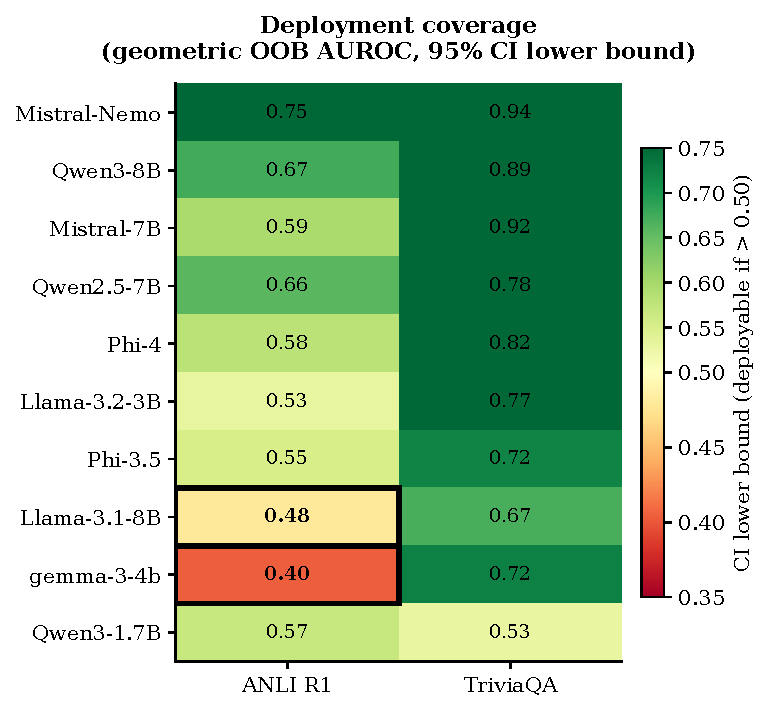
\includegraphics[width=\linewidth]{fig1_coverage.pdf}
\caption{Per-deployment geometric coverage (OOB AUROC, $95\%$ CI lower bound). Boxed deployments are
the two non-deployable ANLI orphans; the weakness is concentrated in one task column.}
\label{fig:cov}
\end{subfigure}\hfill
\begin{subfigure}[t]{0.55\linewidth}
\centering
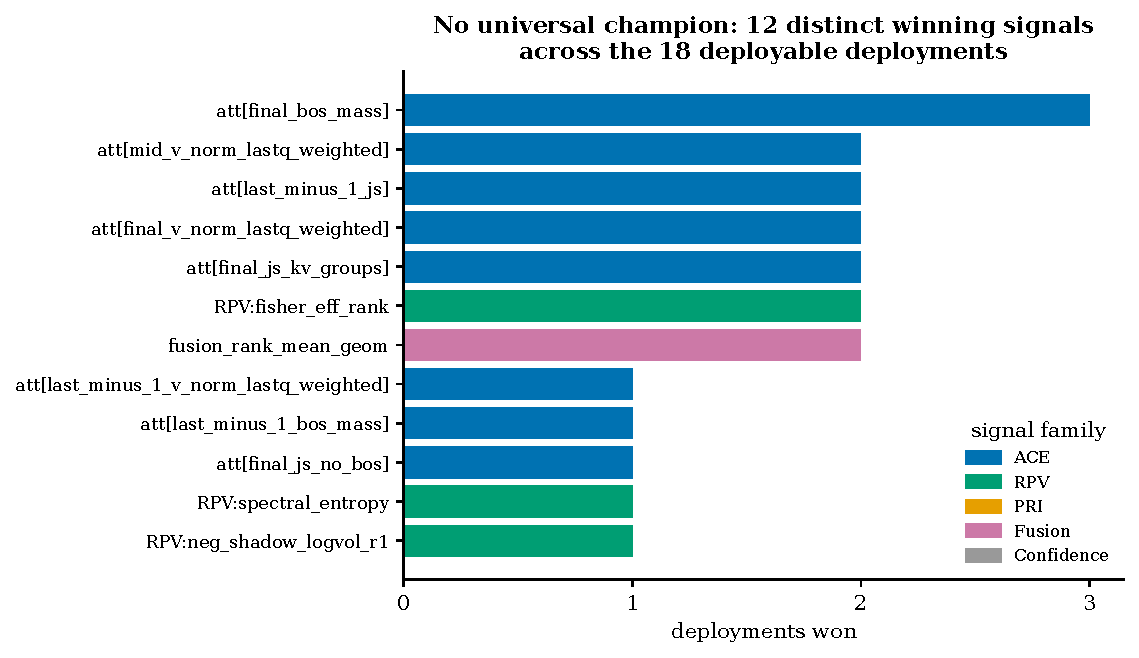
\includegraphics[width=\linewidth]{fig2_winmap.pdf}
\caption{Which signal wins how many deployments: twelve distinct winners across the $18$ deployable
deployments; every geometric family wins somewhere.}
\label{fig:winmap}
\end{subfigure}
\caption{The sealed-core result: (a)~per-deployment coverage and (b)~the heterogeneity of winning
signals behind ``no universal champion.''}
\end{figure}

\paragraph{No universal champion.} Across the $18$ deployable deployments, the winning signal is
one of \emph{twelve distinct} signals (Figure~\ref{fig:winmap}): ACE attention dominates, RPV
covers four deployments where attention does not, and a fusion signal wins two outright. The
families corroborate one another, yet each wins somewhere; no single signal generalizes as the
\emph{best} choice.


\begin{table}[tbp]
\centering
\caption{Panel glossary --- decoding the signal names in Figure~\ref{fig:winmap}. Each winning
signal is a (layer, statistic) pair read at the commit position (step~0). \emph{Layer prefixes:}
\texttt{final} = last layer, \texttt{last\_minus\_1} = penultimate, \texttt{mid} = middle.}
\label{tab:glossary}
\footnotesize
\begin{tabular}{lll}
\toprule
Statistic & Family & What it reads at the commit position \\
\midrule
\texttt{bos\_mass}                 & ACE        & attention mass on the begin-of-sequence (sink) token \\
\texttt{v\_norm\_lastq\_weighted}  & ACE        & value-vector norm weighted by the committing query's attention \\
\texttt{js}                        & ACE        & inter-head attention disagreement (Jensen--Shannon radius) \\
\texttt{js\_no\_bos}               & ACE        & inter-head disagreement with the sink token removed \\
\texttt{js\_kv\_groups}            & ACE        & disagreement across grouped-query (KV) groups \\
\texttt{fisher\_eff\_rank}         & RPV        & effective rank of the readout (softmax-Fisher) spectrum \\
\texttt{spectral\_entropy}         & RPV        & normalized entropy of the readout spectrum \\
\texttt{neg\_shadow\_logvol\_r1}   & RPV        & rank-1 readout ``pseudo-volume'' (spread off the top axis) \\
\texttt{null\_ratio}               & PRI        & residual motion lying off the readout's top direction \\
\texttt{fusion\_rank\_mean\_geom}  & Fusion     & rank-mean of one representative per family (ACE, PRI, RPV) \\
\texttt{surprise}, \texttt{p\_max} & Confidence & token surprise / maximum output probability \\
\bottomrule
\end{tabular}
\end{table}

\paragraph{But a universal above-chance floor.} A pre-registered leave-one-model-out probe asks a
different question: whether \emph{one fixed} signal, chosen without seeing the held-out model,
beats chance there. The cross-locus \emph{fusion} aggregate does. It clears the registered
$\geq 8/10$ bar on both tasks ($9/10$ on ANLI, $10/10$ on TriviaQA; Figure~\ref{fig:floor}). The
mechanism is unremarkable: a rank-mean of several signals is variance-reduced, so it is the most
cross-model-stable signal even though it rarely wins any single deployment outright. The floor is
also modest. The bar is ``beats chance'' ($0.55$), and strength is heterogeneous: held-out AUROC
spans $0.54$--$0.95$, weaker on ANLI, stronger on TriviaQA.


\paragraph{Task transfer is partial.} Applying each model's per-task winner to the \emph{other}
task gives a median transfer AUROC of $0.67$, above the $0.55$ floor on $85\%$ of transfers. So
per-\emph{model} calibration is a decent --- not perfect --- cross-task proxy: the per-task
requirement is partial, not absolute.

\paragraph{Label cost.} E3 evaluates budgets $n\in\{50,100,150\}$. ANLI subsamples independent rows; TriviaQA draws
complete two-row question stems, so a paired stem is never split. Mean geometric deployability
rises $0.44\rightarrow0.66\rightarrow0.79$, while the full panel rises
$0.46\rightarrow0.71\rightarrow0.81$ (Figure~\ref{fig:labeleff}). The curve is still rising at the
largest measured budget, $n=150$; no $n=200$ E3 point exists. Thus $150$ labels is a measured lower
bound, not an estimated knee.

\begin{figure}[tbp]
\centering
\begin{subfigure}[t]{0.49\linewidth}
\centering
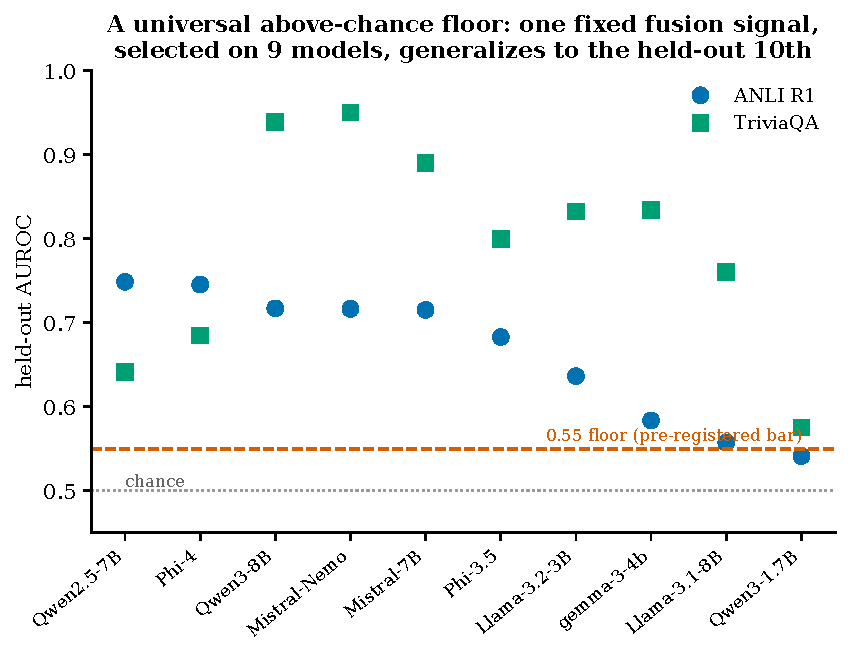
\includegraphics[width=\linewidth]{fig4_universality_floor.pdf}
\caption{Universality floor: the fixed fusion signal, selected on nine models, evaluated on the
held-out tenth. Almost all points clear the pre-registered $0.55$ floor --- the first evidence
\emph{for} partial universality in this program.}
\label{fig:floor}
\end{subfigure}\hfill
\begin{subfigure}[t]{0.49\linewidth}
\centering
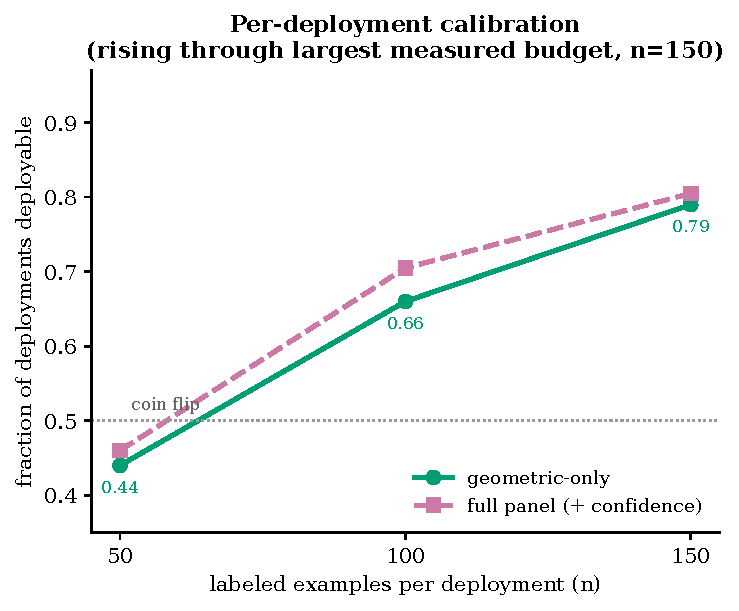
\includegraphics[width=\linewidth]{fig3_label_efficiency.pdf}
\caption{Label-efficiency: fraction of deployable deployments vs.\ labels per deployment ($10$
repeats, $1000$ bootstraps). ANLI subsamples rows; TriviaQA subsamples complete two-row stems, while
the nested OOB bootstrap remains row-level. Geometric-only tracks the full panel within a few points.}
\label{fig:labeleff}
\end{subfigure}
\caption{Cross-model behavior of the selector on the sealed tasks: (a)~the leave-one-model-out
universality floor and (b)~label efficiency.}
\end{figure}

\FloatBarrier
\section{The registered BENCH extension: calibration transfers, orientation does not}
\label{sec:bench}

The sealed run scored two benchmarks across ten open-weight models and reached a two-part reading:
the per-deployment selector is nearly always deployable, but no single commit-moment signal is
universally best. It left two questions open. First, both sealed benchmarks are
\emph{entailment/answer-correctness} tasks; whether the floor reaches a different hallucination
family---judging whether a candidate answer is \emph{faithful to supplied source knowledge}---was
untested. Second, and more consequentially for a deployer, the sealed run only ever calibrated
\emph{per model}; it never asked whether a single frozen detector could ship to a model it was not
tuned on. A universal floor under per-model calibration is a scientific statement; a transferable
fixed detector is a product---and the sealed run could not separate them.

The registered extension (``BENCH'') adds six tasks---HaluEval QA / dialogue /
summarization~\cite{halueval}, ANLI~R2~\cite{anli}, and fresh-draw re-tests of ANLI~R1 (at
$5\times n$ on the train distribution---by registration, \emph{not} a same-distribution
replication) and paired TriviaQA~\cite{triviaqa}---and pre-registers a conjunction that forces the
calibration-versus-transfer distinction into the open, two replication endpoints with their own
bar, and an orphan probe. This section reports the complete extension: every registered endpoint
(A1, A2, B1-procedural, B1-valid, B2) and the exploratory breadth cells. Nothing in it enters or
alters the sealed $18/20$ verdict, which stands as sealed.

\paragraph{Two repairs, disclosed.} Two defects were fixed \emph{before} any strict cell completed,
both filed as numbered amendments in the pre-registration lineage. The transfer estimator's
hard-coded input-version string was synchronized to the current normalizer spec; and the
label-efficiency subsampler, which drew independent rows, was corrected to draw complete stems on
grouped tasks. Both predate every registered metric and alter neither the A1/A2 definitions nor their
bars; the second touches only the descriptive, non-gating label-efficiency analysis.

\subsection{The registered design: three families, five endpoints}

The extension freezes three task families with different epistemic standing (Table~\ref{tab:families}). Family-C cells carry
no bars and, by registration, may narrow but never upgrade any headline claim; ANLI~R2 in
particular is registered as robustness-only and may not be cited as a new benchmark.

\begin{table}[tbp]
\centering\small
\begin{tabular}{@{}p{0.17\linewidth}p{0.28\linewidth}p{0.14\linewidth}p{0.26\linewidth}r@{}}
\toprule
Family & Task & Status & $n$ (rows) & Cells \\
\midrule
A --- breadth      & \texttt{halueval\_qa}            & confirmatory & $1000$ ($500$ stems $\times$ $2$) & $10$ \\
B --- replication  & \texttt{anli\_r1\_rep}           & confirmatory & $1000$ ($500/500$, ungrouped)     & $10$ \\
B --- replication  & \texttt{triviaqa\_paired\_rep}   & confirmatory & $1000$ ($500$ q $\times$ $2$)     & $10$ \\
C --- exploratory  & \texttt{anli\_r2}                & robustness   & $1000$ ($500/500$, ungrouped)     & $10$ \\
C --- exploratory  & \texttt{halueval\_dialogue}      & length-gated & target $1000$                     & $\leq 10$ \\
C --- exploratory  & \texttt{halueval\_summarization} & length-gated & target $1000$                     & $\leq 10$ \\
\bottomrule
\end{tabular}
\caption{The six registered tasks. The confirmatory denominator is exactly $30$ cells (families
A$+$B); a family-A/B cell that cannot run is a reported failure, never a substitution.}
\label{tab:families}
\end{table}

Endpoints A1 and A2 score family A; B1-procedural and B1-valid score the $20$ family-B cells
against a $\geq 17/20$ bar (procedural: row bootstrap unit, the unit the sealed gate used; valid:
cluster unit on grouped tasks---only B1-valid may support replication-strength language); B2 is a
registered probe of the two sealed ANLI orphans on fresh data, reported either way. Every cell
uses the same $29$-signal panel as the seal---ACE attention morphology~\cite{ace}, the PRI
null-ratio~\cite{pri}, the RPV readout spectrum~\cite{rpv}, confidence, and two fusion
aliases---under the same nested-OOB selector.

The two family-A endpoints score the same ten models on HaluEval-QA ($n{=}1000$ rows per model,
drawn as $500$ question stems $\times$ two candidates each; $500$ faithful, $500$ hallucinated;
balanced). For \textbf{A1},
the bootstrap unit is the \emph{question stem} ($500$ clusters), not the row---the conservative
choice on paired data. \textbf{A2} uses no bootstrap: it rank-transforms the frozen fusion score
within each model, fits one sign on the concatenated rows of the nine training models, and reports
a \emph{point} AUROC on the held-out tenth; no A2 confidence interval was pre-registered. Every A2
fold scores the same $1000$ items per model---the holdout is over \emph{models}, not items. Both
endpoints carry a registered bar of $\geq 8/10$. A1 lets each model select its own cell and its own
orientation from its own labels (a statement about \emph{calibration}); A2 freezes one cell
(\texttt{fusion\_rank\_mean\_geom}) and one sign and applies it blind, leave-one-model-out (a fixed
\emph{scoring rule}, point AUROC). The full HaluEval-QA floor claim requires \emph{both}.

\subsection{A1 passes: the floor reaches HaluEval-QA under calibration}

Under per-model calibration, all ten models are deployable: A1 is $10/10$ against its $\geq 8/10$
bar. Every model clears its controls, no cell drops a sample, and no model emits a non-canonical
commitment on HaluEval-QA. The cohort's \emph{weakest} stem-cluster geometric OOB lower bound is
$0.6705$ (\texttt{Qwen3-1.7B}); the rest sit comfortably higher. A1 alone licenses only the
calibration half of the registered claim; under the frozen language rule the extension's overall
verdict is that the floor \emph{partially extends} to HaluEval-QA, with A2 (next subsection) named
as the failing endpoint. (In the A1 sense here, ``floor'' means per-deployment-calibrated
deployability; the fixed-fusion leave-one-model-out floor established on the sealed tasks above is
exactly the object A2 tests---and rejects---on this task.)

Notably, A1 selects \emph{eight distinct winning cells} across the ten models. There is already no
universal \emph{best} cell here---the very pattern the sealed run reported on the original two
benchmarks, now reproduced on a third hallucination family.

\subsection{A2 fails: orientation does not transfer}

The stronger endpoint fails. With the cell and sign frozen and applied blind, A2 clears the bar on
only $6/10$ holdouts (\texttt{aborted=false}; Fig.~\ref{fig:a2}). The pre-registered A1$\wedge$A2 conjunction is
therefore \textbf{not satisfied}. In the registration's frozen wording, the floor \emph{partially
extends} to HaluEval-QA, with A2 the failing endpoint: per-model calibration is licensed, and
shipping this frozen cell-and-sign to an uncalibrated model is not.

\begin{table}[tbp]
\centering
\begin{tabular}{@{}lccc@{}}
\toprule
Held-out model & Pooled sign & Blind AUROC & $>0.55$? \\
\midrule
Llama-3.2-3B      & $-1$ & 0.873 & \checkmark \\
gemma-3-4b        & $-1$ & 0.850 & \checkmark \\
Llama-3.1-8B      & $-1$ & 0.825 & \checkmark \\
Phi-4-mini        & $-1$ & 0.724 & \checkmark \\
Qwen3-8B          & $-1$ & 0.583 & \checkmark \\
Qwen3-1.7B        & $-1$ & 0.577 & \checkmark \\
\addlinespace
Phi-3.5-mini      & $-1$ & \textbf{0.394} & --- \\
Qwen2.5-7B        & $-1$ & \textbf{0.276} & --- \\
Mistral-Nemo      & $-1$ & \textbf{0.206} & --- \\
Mistral-7B        & $-1$ & \textbf{0.174} & --- \\
\bottomrule
\end{tabular}
\caption{A2 leave-one-model-out transfer on HaluEval-QA. The pooled training sign is $-1$ in every
fold. Six holdouts exceed the registered $0.55$ threshold; four fall far below chance. These are
point AUROCs on $n{=}1000$ (no interval was registered for A2), so ``inversion'' names the observed
direction on this fixed dataset---the four failures do not cluster near $0.5$; they sit far below it.}
\label{tab:a2}
\end{table}

\begin{figure}[tbp]
\centering
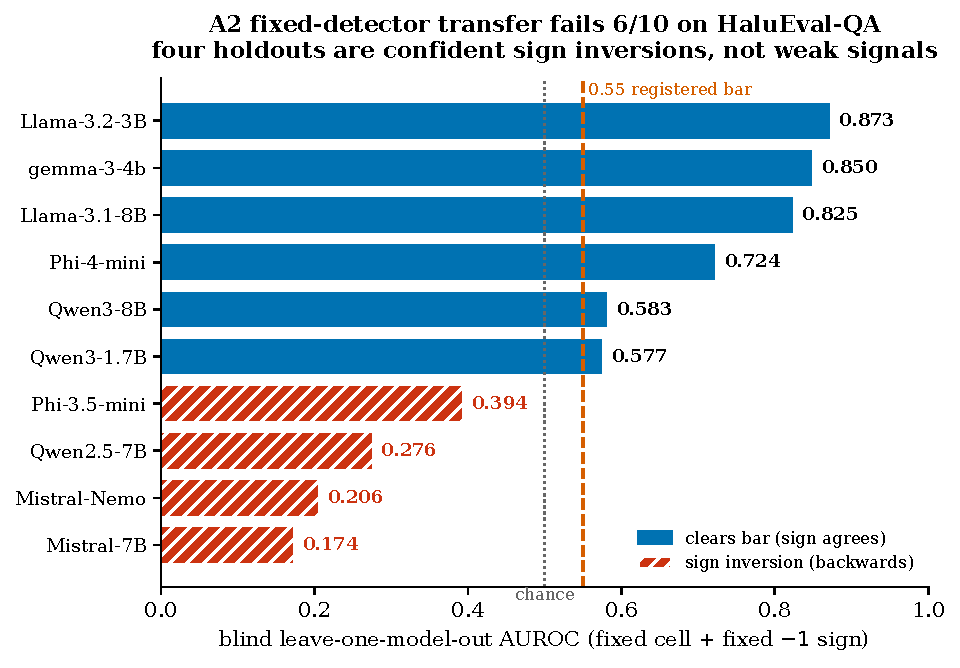
\includegraphics[width=0.56\linewidth]{fig6_a2_transfer.pdf}
\caption{A2 blind leave-one-model-out transfer on HaluEval-QA, sorted by AUROC.
Six holdouts clear the $0.55$ registered bar under the frozen cell and frozen $-1$
sign; four sit \emph{far below} chance. The four low bars (hatched) are not weak
signals---they are sign inversions, the same cell read in the opposite
direction (point AUROCs; no A2 interval was registered). This falsifies only the compound ``\emph{fixed cell plus fixed sign}''
deployment; it does not deny that \texttt{fusion\_rank\_mean\_geom} is a common
informative cell (it clears $0.55$ on all ten once each model's sign is calibrated).
All cells are byte-comparable MLX extractions.}
\label{fig:a2}
\end{figure}

\paragraph{The failure is a sign inversion, not an absence of signal.} The four misses in
Table~\ref{tab:a2} do not cluster near $0.5$; they sit well below it. Each of these models, calibrated
on its \emph{own} labels (the A1 regime), selects the \emph{opposite} orientation ($+1$) from the six
that transfer ($-1$). Under the pooled $-1$ sign they are therefore read upside down. Reversing the
sign rescues each of them---$0.174\!\to\!0.826$, $0.206\!\to\!0.794$, $0.276\!\to\!0.724$,
$0.394\!\to\!0.606$---but \emph{reversal is not an A2 rescue}: choosing to reverse requires knowing the
held-out model's labels, which is exactly the information A1 may use and blind transfer forbids. We
verified the mechanism from the raw score matrices, not the summaries: rebuilding the fused column
per model with the production routine reproduces the registered AUROCs to three decimal places, and
the mean fused rank of faithful-versus-hallucinated examples mirrors exactly---e.g.\ Llama-3.2-3B
$0.62/0.38$ (high~$=$~faithful) against Mistral-7B $0.37/0.63$ (high~$=$~hallucinated).

\paragraph{Observed polarity varies within named families.} Descriptively, Mistral's two checkpoints
share $+1$ and Llama's two share $-1$, while Qwen and Phi split across generations (Qwen2.5 inverts
where both Qwen3 hold; Phi-3.5 where Phi-4 holds). With one or two representatives per subgroup and
generation confounded with tokenizer, architecture, and size, this is incompatible only with a
\emph{simple family-constant orientation in this cohort}---it identifies no cause.

\subsection{B1: the replications miss their bar --- and exactly how}

The registered replication endpoints fail, and the registration requires this miss to be stated
prominently in any publication of the extension. \textbf{B1-procedural and B1-valid both score
$7/20$ against their $\geq 17/20$ bar.} Replication-strength language (``the sealed result
replicates on fresh data'') is therefore \emph{not} licensed, on either bootstrap unit.

The registered verdict is $7/20$ FAIL. The following decomposition is \emph{descriptive}: it
locates where planned cells are lost, and it does not modify or rescue that endpoint:

\begin{table}[tbp]
\centering\small
\begin{tabular}{@{}lc@{}}
\toprule
Layer & Count \\
\midrule
Raw geometry deployable (all profiled replication cells) & $18/18$ \\
Admissible before the systematic-abort cascade & $14/20$ \\
Registered endpoint (after the cascade) & $\mathbf{7/20}$ \\
\bottomrule
\end{tabular}
\caption{B1 descriptive layer decomposition. Geometric OOB CI lower bounds on the $18$ emitted
replication profiles span $0.6577$--$0.9804$ (row unit; $0.6760$--$0.9804$ under the cluster
unit).}
\label{tab:b1}
\end{table}

The registered count falls from $20$ planned cells to $7$ passes in three layers. First, two
\texttt{anli\_r1\_rep} cells are \emph{behavioral} failures: \texttt{Phi-3.5} emits a newline
preamble and \texttt{Qwen2.5-7B} emits the chain-of-thought opener (`` To'') instead of a
canonical YES/NO commitment. Per the registration's own disclosure rule we state plainly that the
commitment normalizer \emph{was amended between smokes and strict cells} (Amendment~A1): the
canonical-commit predicate became ``a non-empty prefix of \texttt{yes} or \texttt{no},'' which
rescues exactly one signature---\texttt{Mistral-7B}'s tokenizer splits \texttt{YES} into
\texttt{Y}+\texttt{ES}, so its first-token \texttt{Y} is a genuine commit misread by the old
exact-form rule---while the newline and `` To'' signatures were explicitly left as failures, with
no behavioral rescue. Those two failures leave $18$ emitted profiles. Second,
\texttt{Qwen3-8B/anli\_r1\_rep} and three \texttt{triviaqa\_paired\_rep} cells fail the
zero-error commitment audit (a single non-canonical commitment in $1000$ disqualifies a cell),
leaving $14/20$ admissible. Third, the three TriviaQA failures (rates $1/1000$, $1/1000$, and
$12/1000$---\texttt{gemma-3-4b} sometimes answers the trivia question instead of judging the
candidate) trigger the frozen systematic-abort rule, which scores all ten TriviaQA cells as
failures, including the seven whose terminal status is OK. The registered endpoint is therefore
$7/20$. The cascade was registered before the data existed and is applied as written; per the
registration's amendment discipline it cannot be softened retroactively, and a successor rule (a
per-cell error budget with a blip-versus-behavior split) exists only as a draft for a
\emph{future} registration (\S~\ref{sec:forward}).

Read precisely: $7/20$ is the registered B1 verdict. The $18/18$ geometric count is a descriptive
decomposition of the profiles that exist (Table~\ref{tab:b1}; Fig.~\ref{fig:panel}), not a
registered rescue endpoint. It shows that the observed loss occurs in behavioral admissibility
and the systematic-abort cascade rather than in the geometry---and it neither licenses
replication-strength language nor alters the FAIL.

\subsection{B2: both sealed orphans deployable on the fresh-draw re-test}

The sealed run left two non-deployable ANLI cells---\texttt{gemma-3-4b/anli} (geometric CI-lo
$0.403$) and \texttt{Llama-3.1-8B/anli}---and the extension registered a probe of those cells on
a fresh $n{=}1000$ draw, reported either way. As the registration itself requires us to say, this
is a \emph{re-test of the sealed construct at $5\times n$ on the noisier ANLI train
distribution}, not a same-distribution replication (the dev split could not supply $1000$ fresh
balanced rows). \textbf{Both pass:} \texttt{gemma-3-4b} reaches a geometric OOB CI lower bound of
$0.772$ and \texttt{Llama-3.1-8B} $0.676$ on \texttt{anli\_r1\_rep}. Under the registered
reading, these passes \emph{narrow} the orphan interpretation by supporting a small-$n$ artifact
component; they do not erase the sealed failures or alter the sealed verdict, which stands as
sealed. The result is descriptively convergent with the separate scale-axis closures reported in
Section~\ref{sec:scale}, but because this comparison changes both sample size and ANLI
split/distribution, it does not isolate sample size as the cause.

\subsection{Exploratory family C: robustness and length-gated coverage (no bars)}

Family-C cells carry no registered bars; by the frozen design they may narrow but never upgrade
any headline claim, and ANLI~R2 is robustness-only. With that standing fixed, the descriptive
picture (Fig.~\ref{fig:panel}):

\begin{figure}[tbp]
\centering
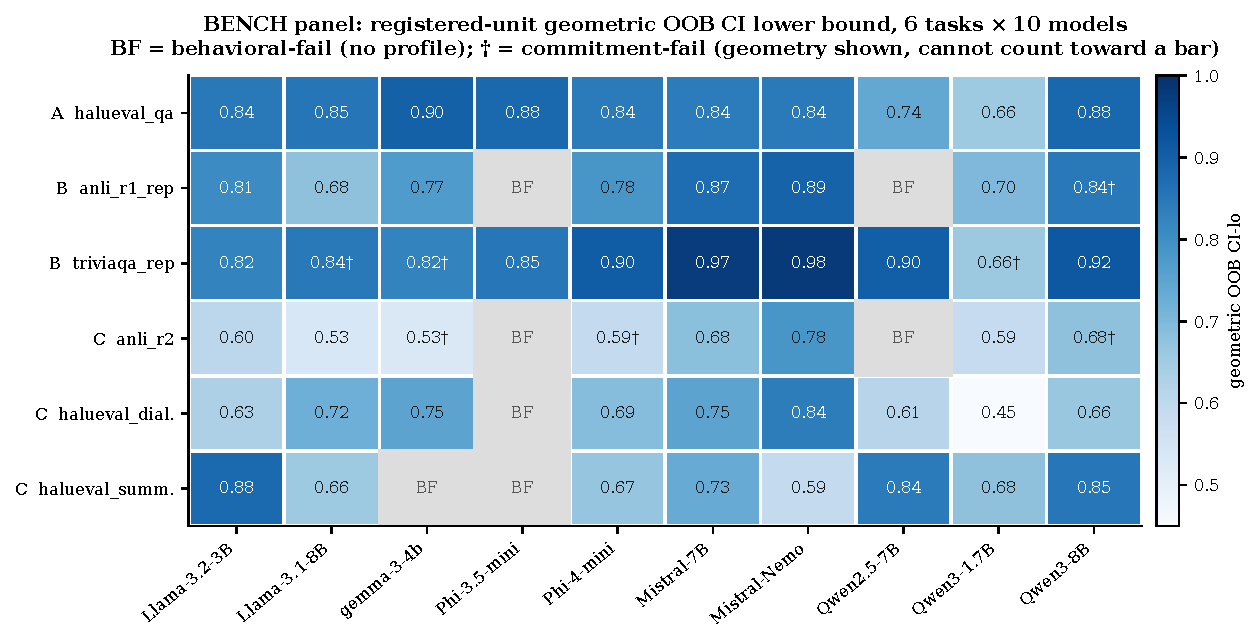
\includegraphics[width=0.66\linewidth]{fig8_bench_panel.pdf}
\caption{The realized $6\times10$ BENCH grid: registered-unit geometric OOB CI lower bound for
all $60$ model--task slots (cluster gate on grouped tasks, row gate on ungrouped). Gray \emph{BF}
cells are behavioral failures for which no profile exists; daggered values are commitment-fail
profiles whose geometry is shown descriptively but cannot count as deployable in a registered
endpoint. Of the $53$ profiles that exist, $52$ are geometrically deployable; this profile-only
total is not a registered endpoint and cannot upgrade a headline claim. The sole geometric miss
is \texttt{Qwen3-1.7B} on \texttt{halueval\_dialogue} ($0.494$).}
\label{fig:panel}
\end{figure}

Descriptively (Fig.~\ref{fig:panel}): \textbf{ANLI~R2} is deployable on every profiled cell but in a
visibly weaker band ($0.528$--$0.782$) than the R1 re-test, as expected for a harder round and
reported as robustness color only. \textbf{HaluEval dialogue/summarization} profile $17/20$ planned
cells ($3$ behavioral failures) with $16/17$ deployable, attention-morphology cells again dominating.
Overall $53$ of $60$ slots produce profiles and $52/53$ are geometrically deployable---an aggregate
that excludes the seven behavioral-fail slots, is not a registered endpoint, and cannot upgrade A1/A2
or B1. \texttt{Phi-3.5} is the behavioral outlier (non-canonical commitment on four of six tasks, an
output-formatting property distinct from its intact geometry).

\subsection{What is and is not universal}

The extension's result must be restated carefully, because it is easy to over- or under-claim.

\begin{itemize}
\item There is \textbf{no universal orientation}: the same cell reads faithfulness in opposite
directions across models, and no single sign serves all ten.
\item There is \textbf{no universal best cell}: A1 selects eight distinct winners across ten models.
\item But this is \textbf{not} the absence of a common informative cell. The frozen cell
\texttt{fusion\_rank\_mean\_geom} clears $0.55$ on \emph{all ten} models once each model's sign is
calibrated. A2 rejects the compound deployment claim ``\emph{fixed cell plus fixed sign},'' not the
identity of the cell.
\end{itemize}

The practical reading is blunt: a commit-moment faithfulness monitor can be built for any of these
ten models, but it needs a labeled calibration set from \emph{that} model to fix its orientation.
The one drop-in detector this run pre-registered---the obvious candidate, the cell that is
informative on all ten---does not transfer unseen; the run tested no other fixed detector. This
sharpens rather than contradicts the sealed thesis: the universal object is the \emph{fitting
procedure}, not any fixed signal, and now not even a fixed \emph{orientation}.

\paragraph{Label cost on the new task.} The sealed label-efficiency analysis above is measured on
the sealed ANLI/TriviaQA cells---\emph{not} on HaluEval-QA---and only at budgets
$n\in\{50,100,150\}$, where the curve is still rising at the largest budget. A1 here calibrates on
$1000$ rows ($500$ stems) per model, which is an upper bound, not a cost estimate. A
\emph{descriptive, post-hoc} sweep over the published HaluEval-QA matrices supplies the
lower-bound curve (production label-efficiency machinery with stem-aware complete-stem draws;
budgets $\{50,100,150,300,500\}$; specification committed before execution; because the matrices
already existed, this is an estimate, not a registered endpoint, and it alters no A1/A2 verdict).
The curve saturates early: all ten models reach full subsample deployability by $150$ labels and
stay flat through $300$ and $500$---a measured plateau, in contrast to the sealed tasks, where the
curve is still rising at the largest measured budget. Nine of ten are already fully deployable at
$100$ labels; the last to certify is exactly the cohort's weakest A1 cell (\texttt{Qwen3-1.7B}:
$0.2$ of repeats at $50$, $0.9$ at $100$, $1.0$ at $150$). Descriptively, then, HaluEval-QA is a
\emph{cheaper} calibration target than the sealed tasks---roughly $100$--$150$ labels per model to
fix both cell and orientation---though a registered label-cost endpoint would require fresh data.

\subsection{Scope, construct, and limitations of the extension}

Four scope limits bound every claim above. \textbf{Construct:} each HaluEval-QA row supplies a
question, source knowledge, and a candidate answer, and we read geometry at the YES/NO
faithfulness-commit token---this is \emph{recognition} of a presented candidate, not detection of the
model's \emph{own} hallucinations during free generation. \textbf{Stimuli:} the counterfeits are
HaluEval's dataset-synthesized negatives, so generator-specific shortcuts cannot be excluded in
principle. \textbf{Inference:} A1 carries stem-clustered OOB intervals; A2 is a pre-registered point
estimate with no interval, holding out over models, not items. \textbf{Cohort:} ten open-weight
models, $1.7$--$8$B, all 4-bit MLX---``cohort'' is the load-bearing word in every universality
statement.

\subsection{Provenance and honest attestation}

The extension ships with an enforced checksum chain, not a trust-me summary: a manifest
(\texttt{PROVENANCE.json}, schema \texttt{bench-provenance/1.1}) binds a SHA-256 for each of the $53$
matrices and profiles, run sidecars, and lifecycle logs, and a CI verifier fails closed on any
mismatch. Its scope is deliberate---it establishes \emph{repository coherence} (published files match
their declared checksums and pairing), not an execution-time signature, and recomputes no endpoint.
The original detached run's exit status was never captured and is documented as unrecoverable rather
than reconstructed after the fact.

\paragraph{Comparability.} All BENCH cells are reported within a single MLX extraction stack and
are byte-comparable with one another and with the sealed cells. They are \emph{not} pooled with the
non-byte-comparable extension cells of Section~\ref{sec:scale} (GPU/torch scale panels or
reimplemented multimodal extractors), which are sectioned and daggered separately.

\subsection{Forward work}
\label{sec:forward}

Two forward-work documents were drafted at the close of the run, neither applied retroactively. One
proposes a future pre-registration with a per-cell commitment error budget and a widened
acceptable-answer template, to be filed blind before fresh data; it remains a draft. The other
specified a designed-retrospective screen---predictor frozen, discovery task excluded---for a
coincidence: three of the four inverting models overlap a partial-transfer cluster from an earlier
sealed run. Executed exactly as frozen (design hashed before execution), it finds \emph{no}
association (Fisher exact two-sided $p=0.50$; the ``distinctive'' orientation is the cohort norm,
$7/9$). The overlap is a coincidence at that resolution; being retrospective it cannot exclude a
finer sub-family, but it removes the evidence that would have motivated a registered fresh-data
test.

\paragraph{Bottom line.} On a third, independent hallucination family, the registered verdict is
that the floor \emph{partially extends}: calibration holds ($10/10$) and the one pre-registered
fixed orientation does not transfer ($6/10$, the named failing endpoint), failing by inversion
rather than by noise. The replication bar is missed ($7/20$, a commitment-protocol cascade over
descriptively intact geometry), and both sealed orphans pass their registered re-test probe. The
signal is real on all ten models; what failed is the one label-free way this run pre-registered
to ship it.

\paragraph{Artifacts.} The registered matrices, profiles, endpoint records
(\texttt{SUMMARY.json}, \texttt{A2\_REGISTERED.json}), the provenance manifest and verifier, and
the pre-registration lineage are published at
\url{https://github.com/flowstyleliving/commit-confluence} (\texttt{stage\_b/profiles\_bench/}).

\FloatBarrier
\section{Post-seal extension: scale and generation close the orphan}
\label{sec:scale}

The strict-product falsification above rests on two orphan deployments; we ask whether they are
\emph{permanent} blind spots or artifacts of model capacity. This is a pre-registered, out-of-sample
extension run \emph{after} the seal (predictions frozen before any metric; same fresh data, seed,
panel, and selector; module hashes identical to the seal, so it is byte-comparable). It does
\textbf{not} enter or alter the sealed $18/20$.

We add two models on the same two tasks at $n{=}200$: \texttt{gemma-3-12b} (the \emph{scale} axis ---
same generation as the orphan \texttt{gemma-3-4b}, $\sim\!3\times$ the parameters) and
\texttt{Qwen2.5-14B} (a non-gemma \emph{family} control). All four new cells are deployable
(Table~\ref{tab:ext}), and the \texttt{gemma-3-4b/ANLI} orphan --- which failed
\emph{both} endpoints in the seal (geometric CI-lo $0.403$) --- is recovered by scale
(\texttt{gemma-3-12b/ANLI} CI-lo $0.71$). The family control passes ANLI ($0.77$), ruling out a generic
``12--14B needed for ANLI'' effect: the failure was the \emph{small} gemma specifically. Across these
byte-comparable cells every new winner is an ACE attention signal and confidence never wins alone,
consistent with the main panel.

\begin{table}[tbp]
\centering
\caption{Post-seal scale/family/generation extension ($n{=}200$, strict, controls pass): geometric-only
OOB AUROC 95\% CI lower bound (deployable if $>0.50$). Sealed \texttt{gemma-3-4b/ANLI} shown for
contrast. Rows above the rule are byte-comparable to the seal; $\dagger$ marks the generation-axis
cells (\texttt{gemma-4}), which use the same calibrator but a reimplemented extractor and are therefore
\emph{not} byte-comparable (see text).}
\label{tab:ext}
\small
\begin{tabular}{llcc}
\toprule
Model & Task & CI-lo & Deployable \\
\midrule
\texttt{gemma-3-4b} (sealed orphan) & ANLI R1  & $0.403$ & no \\
\texttt{gemma-3-12b}                & ANLI R1  & $\mathbf{0.71}$ & \textbf{yes} \\
\texttt{gemma-3-12b}                & TriviaQA & $0.93$ & yes \\
\texttt{Qwen2.5-14B}                & ANLI R1  & $0.77$ & yes \\
\texttt{Qwen2.5-14B}                & TriviaQA & $0.60$ & yes \\
\midrule
\texttt{gemma-4-12b}$^\dagger$      & ANLI R1  & $0.69$ & yes \\
\texttt{gemma-4-12b}$^\dagger$      & TriviaQA & $0.75$ & yes \\
\bottomrule
\end{tabular}
\end{table}

\paragraph{Interpretation (tested).} A head-\emph{resolution} hypothesis---\texttt{gemma-3-4b} has
$8$ heads / $4$ KV-groups vs.\ $16$ / $8$ for \texttt{gemma-3-12b}---is directly refuted by a
within-model ablation: recomputing the ACE statistics over the smaller head budget leaves ANLI
deployable (CI-lo $0.71\!\to\!0.67$), only ${\sim}11\%$ of the $0.31$ gap. Recovery is driven by
representation quality, not head count.

\paragraph{Generation axis (gemma-4).} The remaining axis---a newer model \emph{generation}---is now
also testable, with a caveat. \texttt{gemma-4}'s \texttt{gemma4\_unified} architecture is unsupported by
the inference stack the seal used, so we extract its panel through a separate implementation: a
different loader plus a from-scratch attention recompute, the latter validated against the model's own
output projection to numerical identity ($\cos{=}1.0$). The same calibrator and selector then score it.
These two cells are therefore \emph{not} byte-comparable to the seal and are reported as a standalone
generation-axis point, never pooled with the byte-comparable cells above (Table~\ref{tab:ext},
daggered). With that caveat, \texttt{gemma-4-12b} is deployable on \emph{both} tasks (ANLI CI-lo $0.69$,
TriviaQA $0.75$). The orphan does \emph{not} reappear a generation later: \texttt{gemma-4-12b}/ANLI
($0.69$) sits beside \texttt{gemma-3-12b}/ANLI ($0.71$), both far above the sealed
\texttt{gemma-3-4b}/ANLI ($0.403$). Taken with the scale result, this localizes the orphan to small
\emph{gen-3} capacity specifically, not to the gemma lineage. One difference from the byte-comparable
cells: both \texttt{gemma-4} winners are the cross-locus \emph{fusion} signal rather than a solo ACE
attention signal---plausibly reimplementation drift in the attention statistics, and a reason not to
over-read the per-signal identity of these two non-byte-comparable cells.

A further out-of-stack extension reaches still larger models through a GPU implementation: torch with
4-bit \texttt{bitsandbytes}, the output embedding held in floating precision, and the attention capture
again validated against the model's own output projection to $\cos{=}1.0$. These cells are likewise
\emph{not} byte-comparable to the seal and are never pooled with it. Two observations follow. First,
the second sealed ANLI orphan resolves exactly as the first did. \texttt{Llama-3.1-8B}/ANLI fails in
the seal, but \texttt{Llama-3.3-70B}/ANLI is deployable (CI-lo $0.70$); both sealed ANLI orphans are
therefore small-model artifacts, now witnessed across two independent families. Second, and more
cautionary for any universality claim, \texttt{Llama-3.3-70B} is deployable on both tasks (ANLI
$0.70$, TriviaQA $0.79$), yet \emph{both} of its winners are readout-geometry signals at the first
generated token---not the ACE attention morphology that wins every byte-comparable cell. The locus
that carries the signal is thus family-dependent: attention-side for Qwen, readout-side for Llama.
This is why we scope the ``ACE attention wins'' statement to the byte-comparable cells and let the
cross-locus panel, rather than any single signal, be the object that transfers across models.

\paragraph{Precision deconfound.} A pre-registered precision ladder (\texttt{Qwen2.5-7B} across
\texttt{nf4}/\texttt{int8}/\texttt{bf16}/\texttt{fp32}; \texttt{Qwen2.5-32B} across the first three)
tests whether the signal is rounding noise. Judged on fixed cells rather than the selection-noisy
argmax winner, robust signals keep direction and strength across rungs, and the registered
quantization-artifact falsifier (a large \texttt{nf4}$\to$\texttt{bf16} drop) is not observed; the
ladder also caught a mislabeled-precision provenance bug whose true-\texttt{nf4} rerun still wins on
ACE attention. The family-dependent locus is thus not a precision artifact.

\FloatBarrier
\section{Discussion}

Neither extreme fits these results. A single universal detector overstates what transfers; the
fallback that nothing transfers understates it. The supported shape is a \emph{floor}, not a
champion: a fixed aggregate beats chance on essentially every unseen model, while peak performance
still requires per-deployment calibration. The registered extension sharpens that boundary from the
transfer side---what carries across models is the \emph{informativeness} of a shared cell, not its
\emph{orientation}---so on a new task family even the floor must be shipped with per-model sign
calibration, and the one label-free deployment this program pre-registered does not survive contact
with unseen models. Two consequences follow for deployment safety. First, sharpening is
per-deployment work throughout: on the sealed tasks the label-efficiency curve is still rising at the
largest measured budget of $150$ labels, while HaluEval-QA certified at $100$--$150$ labels in the
post-hoc estimate of Section~\ref{sec:bench}. Second, a trustworthy monitor must know where it cannot
read: a sealed small-model deployment whose interval does not clear the gate should trigger
abstention, not a confident-looking number---the response that standard benchmark grading is argued
to under-reward \cite{kalai2025hallucinate}. Scale may close such blind spots later, but the monitor
must respect the deployment in front of it.

\paragraph{Limits.} The sealed core is two tasks, ten models, a single commit-moment framing, and
a low ($0.55$) universality bar; the descriptive analyses are non-gating. The registered BENCH
extension adds six task registrations on the same cohort but inherits the framing's limits: its
construct is recognition of a supplied candidate at a YES/NO commit token, not free-generation
hallucination; its counterfeits are dataset-synthesized; and its cohort spans $1.7$--$8$B 4-bit
MLX models, so every universality statement is cohort-scoped. The post-seal scale and precision
extensions are reported for interpretation only---several use a different inference stack and are
non-byte-comparable to the seal---and are not folded into the sealed $18/20$ endpoint. The sealed
orphans show that some exact (model, task, stack) deployments have no certified
commit-moment signal under this panel --- a negative the protocol was designed to be able to
return --- even when larger related models later become readable.

\paragraph{Reproducibility.} The pre-registration, the gated fresh data, and the per-deployment
score matrices are public, and the run was executed from a tagged commit, so the executed code is
byte-identical to the registration; every registered endpoint and descriptive universality probe
re-runs from the repository alone, with no model inference. The BENCH extension follows the same
discipline with its own checksummed artifact tree (\texttt{stage\_b/profiles\_bench/}). Code and
matrices: \url{https://github.com/flowstyleliving/commit-confluence}.

\FloatBarrier
\begingroup\footnotesize
\begin{thebibliography}{99}\setlength{\itemsep}{0pt}\setlength{\parskip}{0pt}
\bibitem{farquhar2024semantic} S.~Farquhar, J.~Kossen, L.~Kuhn, Y.~Gal.
\emph{Detecting Hallucinations in Large Language Models Using Semantic Entropy}. Nature, 2024.
\bibitem{kalai2025hallucinate} A.~T.~Kalai, O.~Nachum, S.~S.~Vempala, E.~Zhang.
\emph{Why Language Models Hallucinate}. arXiv:2509.04664, 2025.
\bibitem{agrawal2024references} A.~Agrawal, M.~Suzgun, L.~Mackey, A.~T.~Kalai.
\emph{Do Language Models Know When They're Hallucinating References?} Findings of EACL, 2024.
\bibitem{wastl2025selfconsistency} M.~Wastl, J.~Vamvas, R.~Sennrich.
\emph{UZH at SemEval-2025 Task 3: Token-Level Self-Consistency for Hallucination Detection}.
SemEval, 2025.
\bibitem{xiao2024sinks} G.~Xiao, Y.~Tian, B.~Chen, S.~Han, M.~Lewis.
\emph{Efficient Streaming Language Models with Attention Sinks}. ICLR, 2024.
\bibitem{binkowski2026sinks} J.~Binkowski, K.~Adamczewski, T.~Kajdanowicz.
\emph{Attention Sinks as Internal Signals for Hallucination Detection in Large Language Models}.
arXiv:2604.10697, 2026.
\bibitem{vazhentsev2025rauq} A.~Vazhentsev et al.
\emph{Uncertainty-Aware Attention Heads: Efficient Unsupervised Uncertainty Quantification for
Large Language Models}. arXiv:2505.20045, 2025.
\bibitem{hu2025harp} J.~Hu, G.~Tu, S.~Cheng, J.~Li, J.~Wang, R.~Chen, Z.~Zhou, D.~Shan.
\emph{HARP: Hallucination Detection via Reasoning Subspace Projection}. arXiv:2509.11536, 2025.
\bibitem{pri} M.~S.~R.~Kitti.
\emph{The Predictive Rupture Index: Commitment-Moment Hallucination Signals (v1--v3)}.
Furnace Research, 2026 (in preparation); code and sealed profiles at
\url{https://github.com/flowstyleliving/commit-confluence}.
\bibitem{ace} M.~S.~R.~Kitti.
\emph{The Attention Commitment Estimator: $W_u$-Free Commitment Morphology}.
Furnace Research, 2026 (in preparation); code and sealed profiles at
\url{https://github.com/flowstyleliving/commit-confluence}.
\bibitem{rpv} M.~S.~R.~Kitti.
\emph{Readout Pseudo-Volume: A Confidence-Independent, $\Delta h$-Free Commitment Signal}.
Furnace Research, 2026 (in preparation); code and sealed profiles at
\url{https://github.com/flowstyleliving/commit-confluence}.
\bibitem{anli} Y.~Nie, A.~Williams, E.~Dinan, M.~Bansal, J.~Weston, D.~Kiela.
\emph{Adversarial NLI: A New Benchmark for Natural Language Understanding}. ACL, 2020.
\bibitem{triviaqa} M.~Joshi, E.~Choi, D.~Weld, L.~Zettlemoyer.
\emph{TriviaQA: A Large Scale Distantly Supervised Challenge Dataset for Reading Comprehension}.
ACL, 2017.
\bibitem{halueval} J.~Li, X.~Cheng, W.~X. Zhao, J.-Y. Nie, and J.-R. Wen.
\emph{HaluEval: A Large-Scale Hallucination Evaluation Benchmark for Large Language Models.}
EMNLP 2023.
\end{thebibliography}
\endgroup

\end{document}
